\documentclass[tikz,border=5pt]{standalone}
\usepackage{tikz}
\usetikzlibrary{positioning,fit,backgrounds,calc,shapes.geometric}
\usepackage{graphicx}
\usepackage{xcolor}

\definecolor{gitopsblue}{RGB}{51,108,229}
\definecolor{manualgray}{RGB}{102,102,102}
\definecolor{metricyellow}{RGB}{251,192,45}
\definecolor{driftred}{RGB}{229,115,115}
\definecolor{okgreen}{RGB}{76,175,80}
\definecolor{metricpurple}{RGB}{156,39,176}

\begin{document}
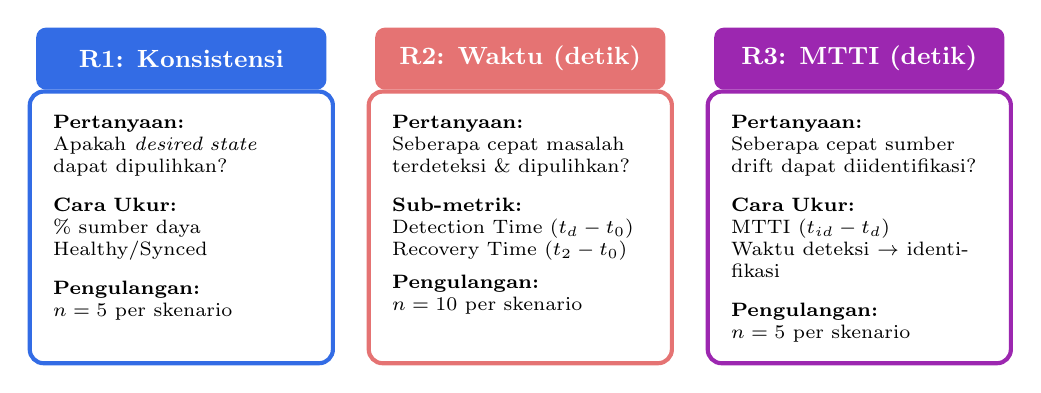
\begin{tikzpicture}[
    node distance=0.42cm and 0.78cm,
    metricbox/.style={rectangle, rounded corners=5pt, draw=#1, fill=white,
                      minimum width=3.85cm, minimum height=3.45cm, align=center,
                      line width=1.5pt},
    metriclabel/.style={rectangle, rounded corners=3pt, draw=#1, fill=#1,
                        text=white, minimum width=3.65cm, minimum height=0.75cm,
                        align=center, font=\small\bfseries, line width=1pt},
    metricdesc/.style={font=\scriptsize, align=left, text width=3.35cm},
    arrow/.style={->, >=stealth, line width=1pt, draw=gray!70}
]

% R1
\node[metriclabel=gitopsblue] (r1label) {R1: Konsistensi};
\node[metricbox=gitopsblue, below=0pt of r1label] (r1box) {};
\node[metricdesc, anchor=north west] at ($(r1box.north west)+(0.2,-0.2)$) {
    \textbf{Pertanyaan:}\\
    Apakah \textit{desired state}\\
    dapat dipulihkan?\\[6pt]
    \textbf{Cara Ukur:}\\
    \% sumber daya\\
    Healthy/Synced\\[6pt]
    \textbf{Pengulangan:}\\
    $n = 5$ per skenario
};

% R2
\node[metriclabel=driftred, right=0.62cm of r1label] (r2label) {R2: Waktu (detik)};
\node[metricbox=driftred, below=0pt of r2label] (r2box) {};
\node[metricdesc, anchor=north west] at ($(r2box.north west)+(0.2,-0.2)$) {
    \textbf{Pertanyaan:}\\
    Seberapa cepat masalah\\
    terdeteksi \& dipulihkan?\\[6pt]
    \textbf{Sub-metrik:}\\
    Detection Time ($t_d - t_0$)\\
    Recovery Time ($t_2 - t_0$)\\[4pt]
    \textbf{Pengulangan:}\\
    $n = 10$ per skenario
};

% R3
\node[metriclabel=metricpurple, right=0.62cm of r2label] (r3label) {R3: MTTI (detik)};
\node[metricbox=metricpurple, below=0pt of r3label] (r3box) {};
\node[metricdesc, anchor=north west] at ($(r3box.north west)+(0.2,-0.2)$) {
    \textbf{Pertanyaan:}\\
    Seberapa cepat sumber\\
    drift dapat diidentifikasi?\\[6pt]
    \textbf{Cara Ukur:}\\
    MTTI ($t_{id} - t_d$)\\
    Waktu deteksi $\to$ identifikasi\\[6pt]
    \textbf{Pengulangan:}\\
    $n = 5$ per skenario
};

\end{tikzpicture}
\end{document}